% \documentclass[reprint, amsmath, amssymb, aps, letterpaper]{revtex4-2}
\documentclass[letterpaper]{article}

\usepackage[letterpaper, margin=1.5in]{geometry} % Set page margins
\usepackage[T1]{fontenc} % Use modern font encodings
\usepackage{microtype} % Improves typography
\usepackage{mlmodern} % Modern font
\usepackage{amsmath} % Advanced math typesetting
\usepackage[dvipsnames]{xcolor} % More colours
\usepackage[colorlinks=true, allcolors=NavyBlue]{hyperref} % Hyperlinks
\usepackage{graphicx} % Include figure files
\usepackage{circuitikz} % Circuit diagrams
\usepackage{subfig} % Subfigures
\usepackage{float} % Better figure placement
% \usepackage{listings} % Code highlighting

\usepackage{graphicx} % Resize figures
\graphicspath{{images/}} % Path to images

\usepackage{listings} % Code highlighting

\usepackage{tikz} % For drawing
\usetikzlibrary{decorations.pathmorphing, patterns}

\usepackage{tabularray} % Better tables
\UseTblrLibrary{booktabs} % Booktabs support for tabularray

\definecolor{codegreen}{rgb}{0,0.6,0}
\definecolor{codegray}{rgb}{0.5,0.5,0.5}
\definecolor{codepurple}{rgb}{0.58,0,0.82}
\definecolor{backcolour}{rgb}{0.95,0.95,0.92}

\lstdefinestyle{mystyle}{
    backgroundcolor=\color{backcolour},   
    commentstyle=\color{codegreen},
    keywordstyle=\color{magenta},
    numberstyle=\tiny\color{codegray},
    stringstyle=\color{codepurple},
    basicstyle=\ttfamily\normalsize,
    breakatwhitespace=false,         
    breaklines=true,                 
    captionpos=b,                    
    keepspaces=true,                 
    numbers=left,                    
    numbersep=5pt,                  
    showspaces=false,                
    showstringspaces=false,
    showtabs=false,                  
    tabsize=2
}

\lstset{style=mystyle}


\begin{document}

\title{Quantum Adder with Quantum Error Correction}

\author{Punit Turlapati}
\maketitle

\begin{abstract}
    An adder circuit adds two binary numbers and outputs the sum and carry bits. When implemented on a quantum computer, the adder circuit is susceptible to errors due to noise and decoherence. Error correction is essential to mitigate these errors and improve the reliability of quantum computations. The Shor code is a quantum error correction code that can correct arbitrary errors on a single qubit. While Shor code does reduce errors, it is not perfect. The chance of getting the incorrect answer is high enough that this circuit should not be used in a real-world application.
\end{abstract}

\section{Introduction}

Quantum computing has emerged as a revolutionary technology that has the potential to solve problems that are impossible for classical computers. Quantum computers use quantum bits, or qubits, which can exist in a superposition of states. This allows quantum computers to perform many calculations simultaneously, leading to exponential speedups over classical computers for certain problems.

One of the fundamental operations in computing is addition. Classical computers use binary numbers, which are represented using binary digits. Binary digits can only have two states, 0 and 1. An adder circuit adds two binary numbers and outputs the sum and carry bits. By chaining together this process, binary numbers of arbitrary lengths can be added.

When the adder circuit is implemented on a quantum computer, the inherently unstable nature of quantum bits introduces errors. The errors can be so significant that they render the computation useless. To mitigate these errors and improve the reliability of quantum computations, error correction is essential. The Shor code is a quantum error correction code that can correct arbitrary errors on a single qubit, which is why it is used in this project. Another limitation was the number of qubits available of IBM Quantum, 126. More complicated error correction codes could not be used due to this limitation.

\section{Theory and Background}

The adder used in this project is a ripple carry adder. It consists of a sum gate, a carry gate, and a carry\(^{\dagger}\) gate. The sum gate calculates the XOR of the two input bits.
\begin{equation*}
    0 \oplus 0 = 0 \qquad\qquad 0 \oplus 1 = 1 \qquad\qquad 1 \oplus 0 = 1 \qquad\qquad 1 \oplus 1 = 0
\end{equation*}

The carry gate manages the overflow from adding two binary digits, letting multi-digit binary addition be possible. It calculates the AND of the two input bits.
\begin{equation*}
    0 \cdot 0 = 0 \qquad\qquad 0 \cdot 1 = 0 \qquad\qquad 1 \cdot 0 = 0 \qquad\qquad 1 \cdot 1 = 1
\end{equation*}

The carry\(^{\dagger}\) gate is the reverse of the carry gate. By chaining together this process, binary numbers of arbitrary lengths can be added.

In order to successfully run the adder on a quantum computer, error correction is essential. By applying the Shor code to the adder circuit, we can mitigate errors and improve the reliability of quantum computations. The Shor code can correct both bit-flip and phase-flip errors on a single qubit. It does this by encoding a single logical qubit into nine physical qubits. First, a singular qubit is represented by three in phase-flip code to correct for phase-flip errors. Then, each one of those three qubits are represented by three qubits in bit-flip code to correct for bit-flip errors. In combination, a phase- or bit-flip in any one of the nine qubits can be corrected.

\section{Methodology}

The code for the adder circuit was written in Qiskit, a Python library for quantum computing. The code is available on GitHub at \url{https://github.com/TheBobTheBlob/Quantum-Adder}.

\subsection{Adder Gates}

The adder circuit consists of three gates. The sum gate, carry gate, and carry\(^{\dagger}\) gate. The carry\(\dagger\) gate is the reverse of the carry gate. The gates are shown in Figure \ref{fig:adder-gates}.

\begin{itemize}
    \item The sum gate consists of two CNOT gates. The circuit requires three qubits. The sum gate calculates the XOR of the two input bits.
    \item The carry gate consists of two Toffoli gates and a CNOT gate. The circuit requires four qubits. The carry gate manages the overflow from adding two binary digits, letting multi-digit binary addition be possible.
    \item The carry\(^{\dagger}\) gate is the reverse of the carry gate. It consists of two Toffoli gates and a CNOT gate, and requires four qubits. It is used to reverse the carry operation.
\end{itemize}

\begin{figure}[H]%
    \centering%
    \subfloat[\centering Sum Gate]{{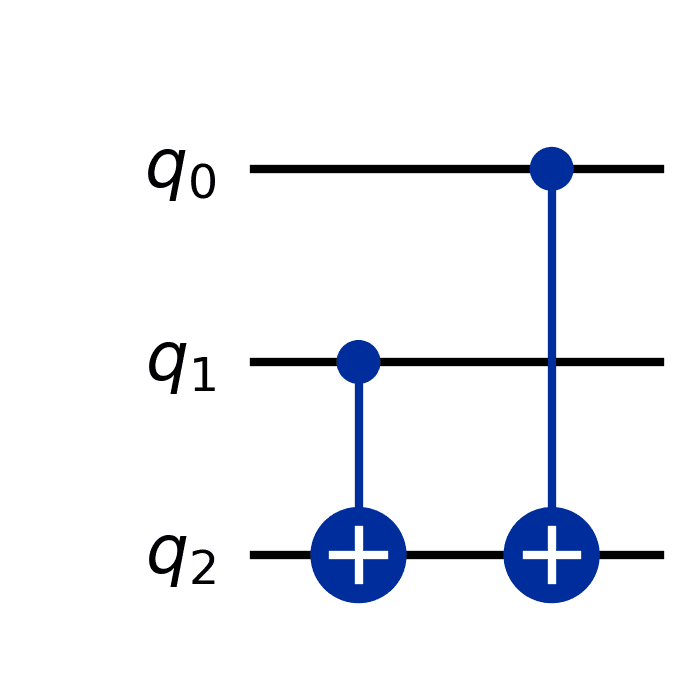
\includegraphics[width=4cm]{sum}}}%
    \qquad%
    \subfloat[\centering Carry Gate]{{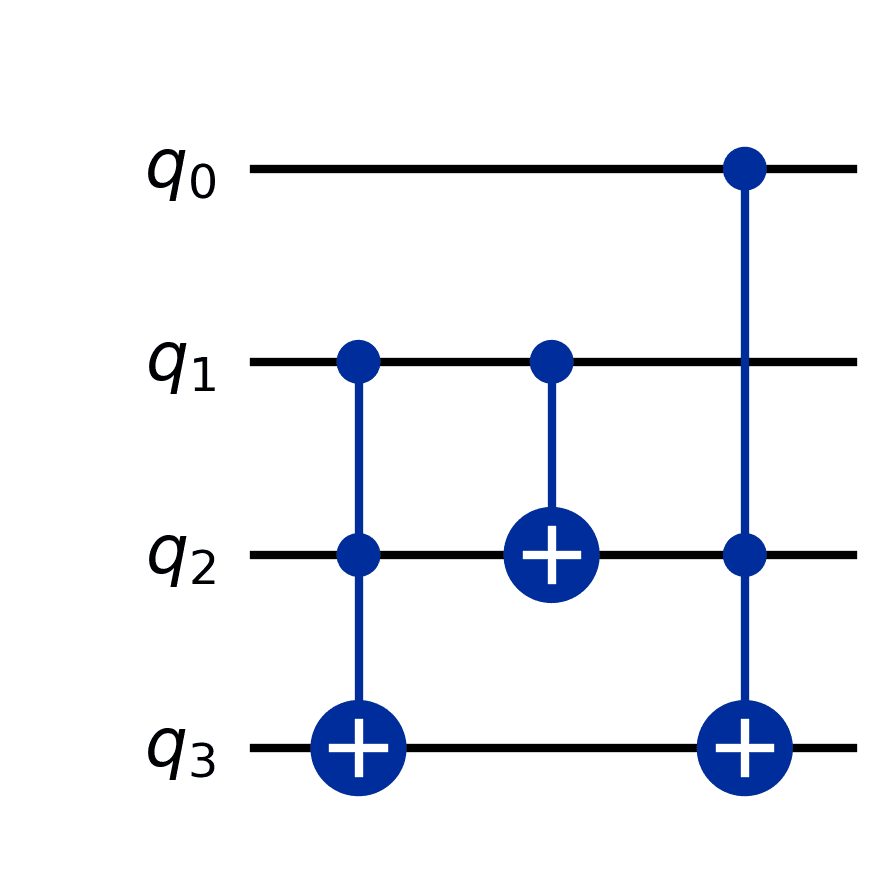
\includegraphics[width=4cm]{carry}}}%
    \qquad%
    \subfloat[\centering Carry\(^\dagger\) Gate]{{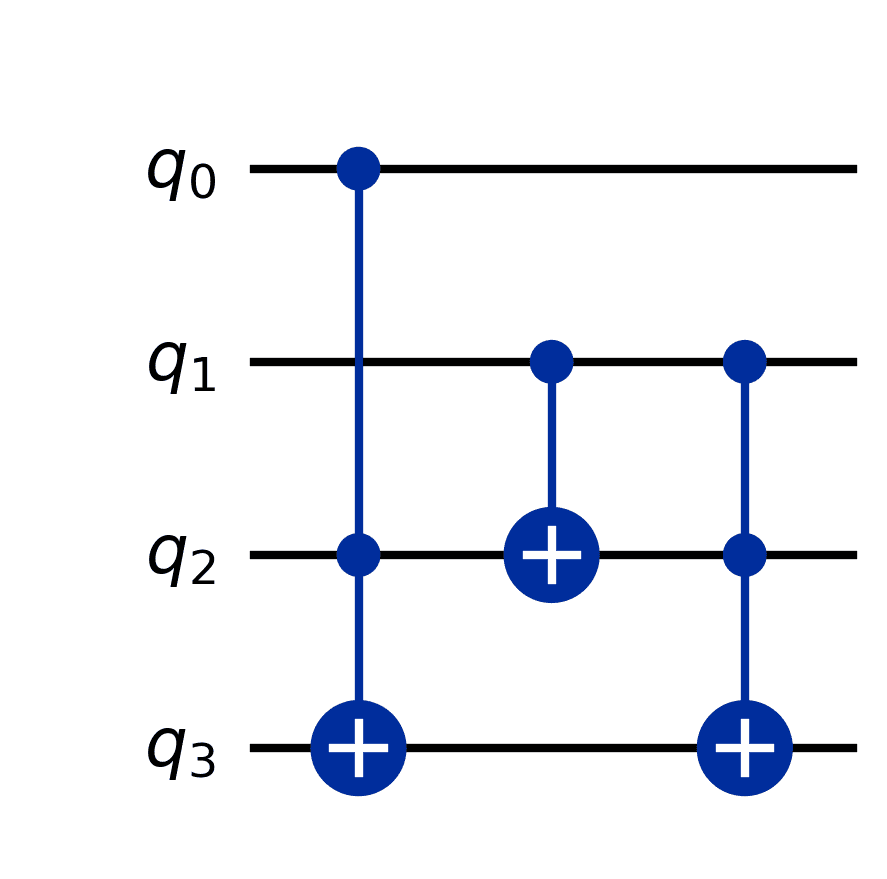
\includegraphics[width=4cm]{reverse_carry}}}%
    \caption{Gates used in the adder circuit.}%
    \label{fig:adder-gates}%
\end{figure}

\subsection{Shor Code}

At the start of the circuit, every bit is encoded into Shor code using the setup circuit. Then when required, the error correction circuit is run, which goes through the nine physical qubits and corrects any arbitrary error in them. Both circuits are shown in Figure \ref{fig:shor-gates}. If necessary, the error correction circuit can be run multiple times on the same set of qubits to re-correct subsequent errors.

\begin{figure}[H]%
    \centering%
    \subfloat[\centering Setup Circuit]{{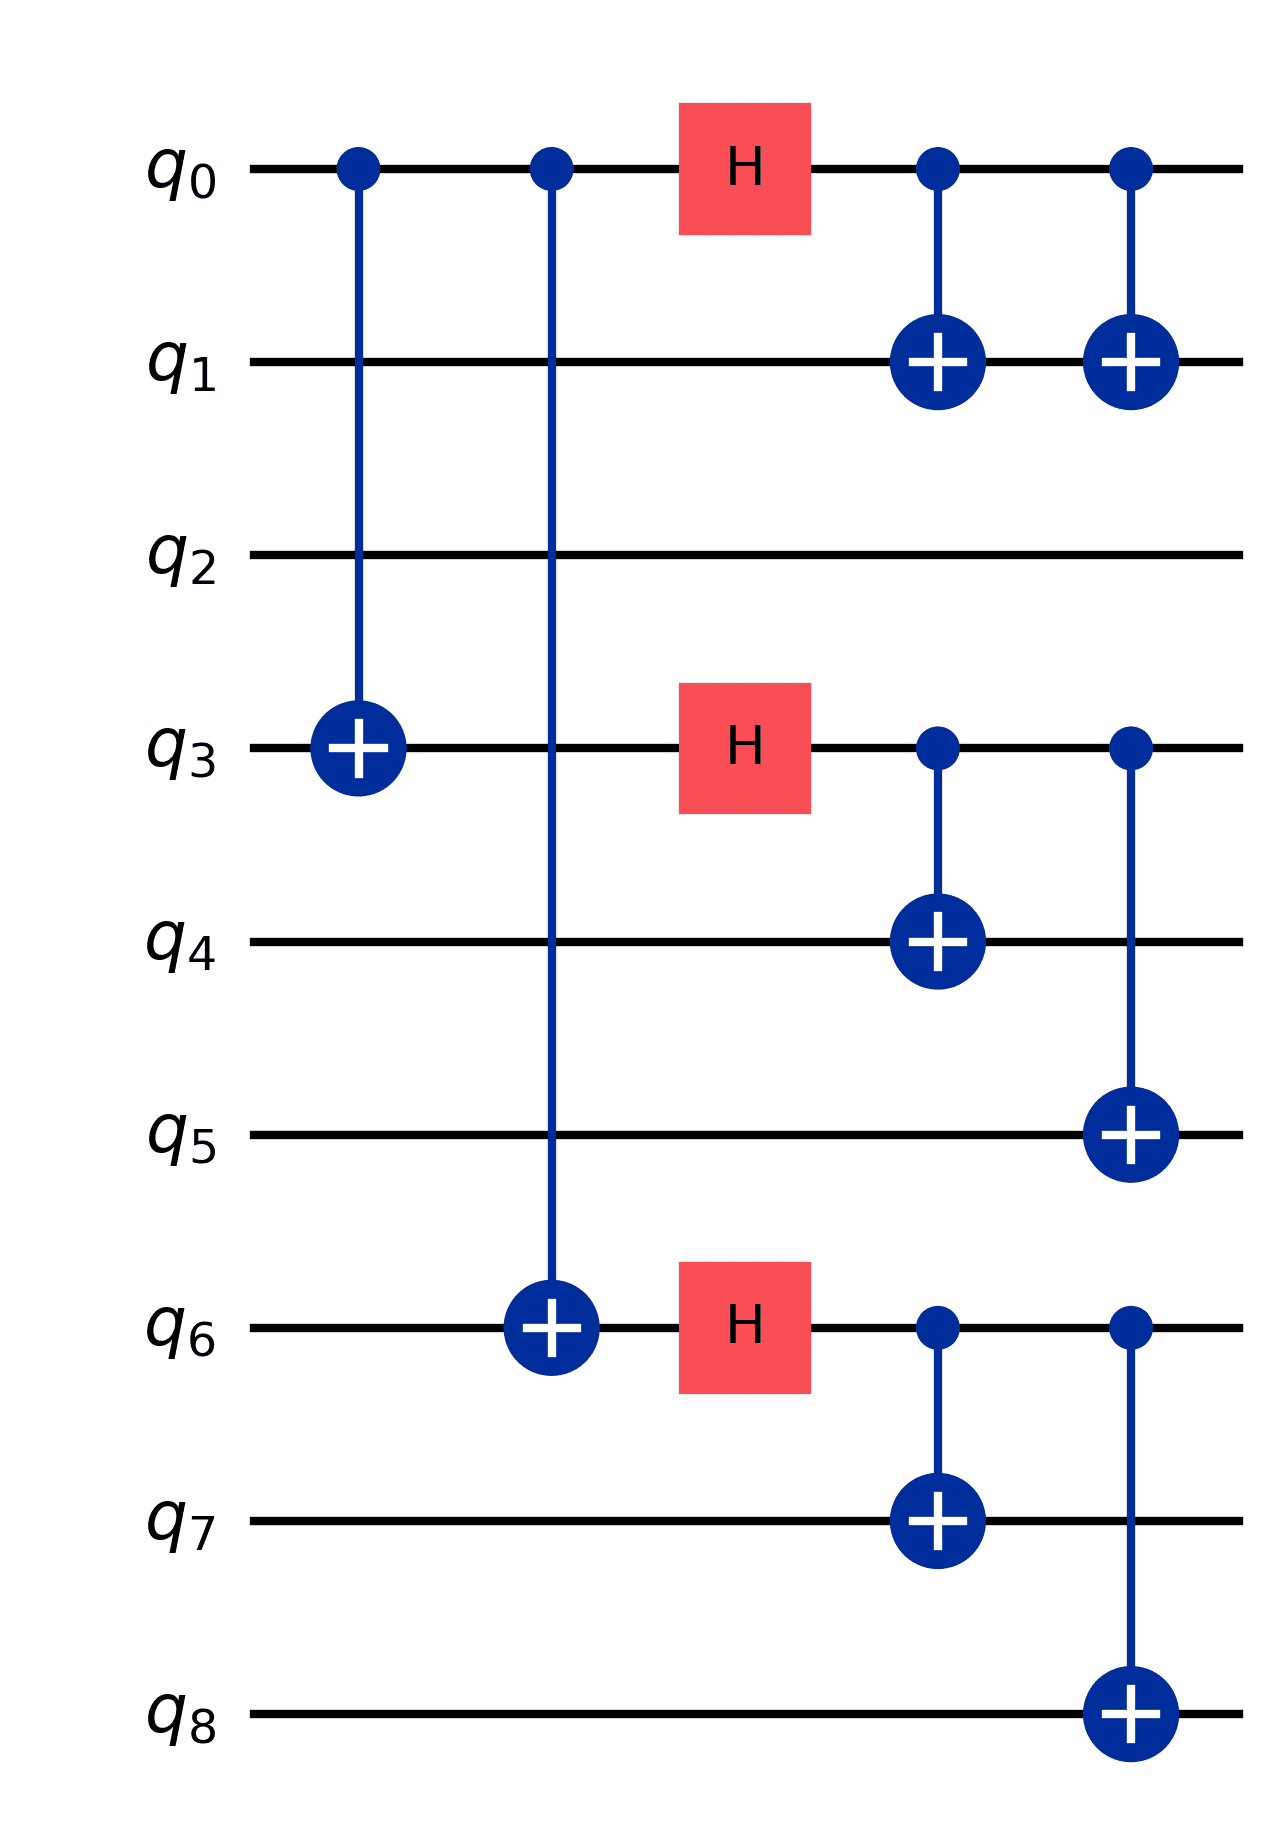
\includegraphics[height=6.25cm]{shor_setup}}}%
    \qquad%
    \subfloat[\centering Error Correction Circuit]{{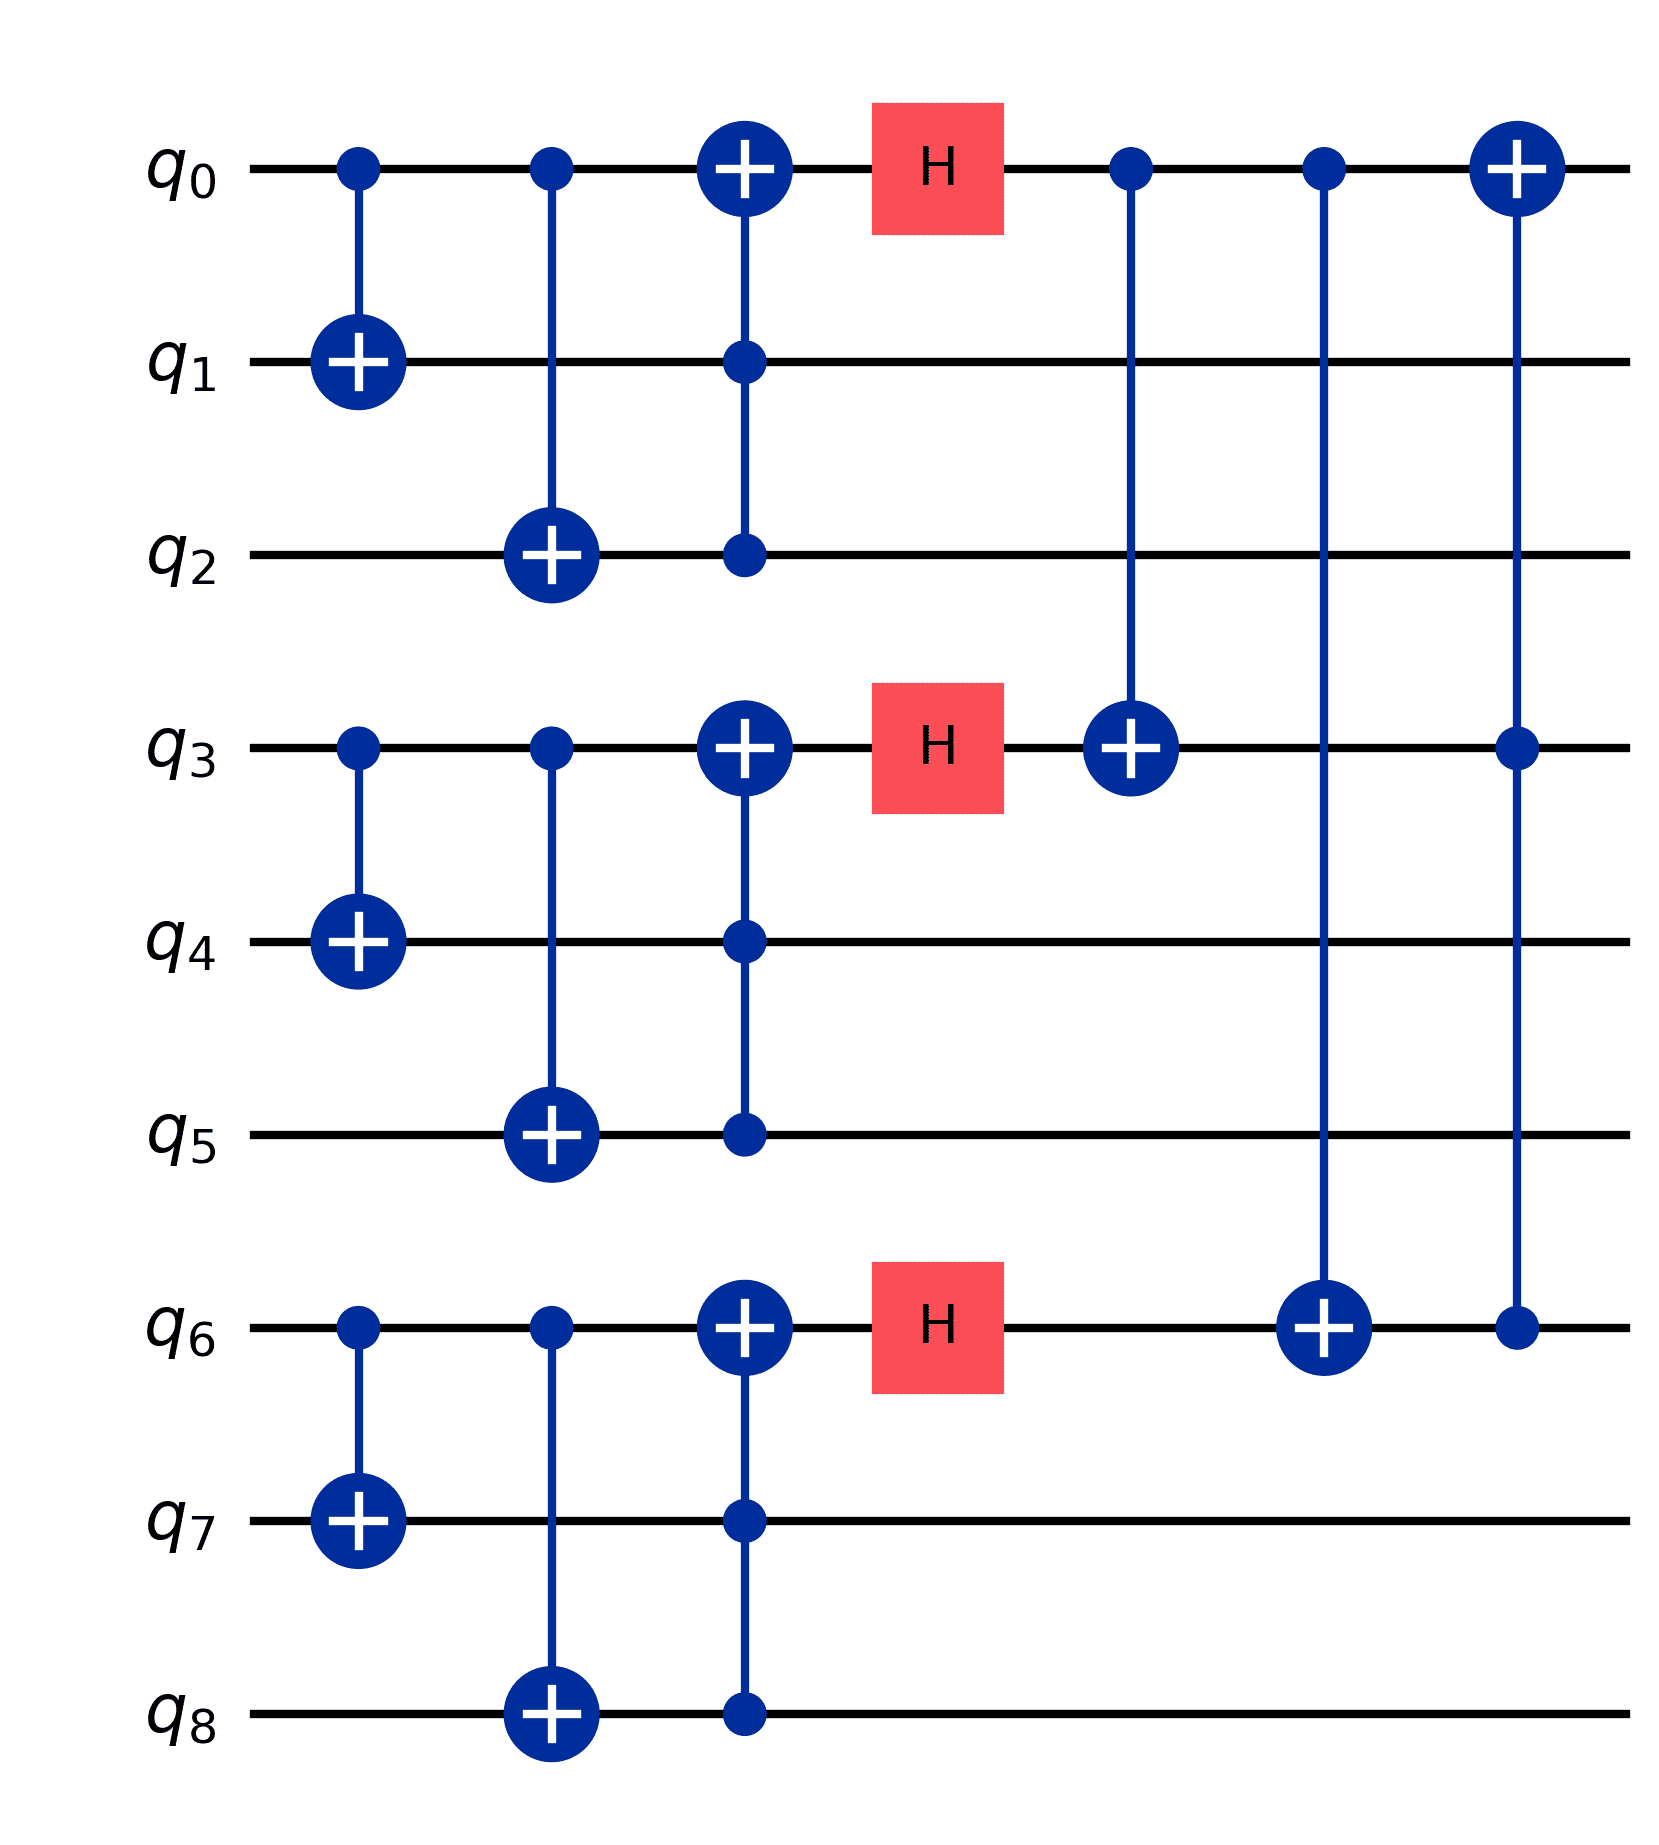
\includegraphics[height=6.25cm]{shor_teardown}}}%
    \caption{The Shor Code}%
    \label{fig:shor-gates}%
\end{figure}

\subsection{Transversal Gates}

When applying a gate to a logical qubit, the gate must be applied to each of the nine physical qubits. However, due to the nature of the Shor code, the physical qubits are in a separate basis when compared to the logical qubit. For example, the transversal version of the X gate is the Z gate. Likewise, the transversal version of the Z gate is the X gate.

\begin{itemize}
    \item The transversal version of the X gate is the Z gate.
    \item The transversal version of the CNOT gate is a flipped CNOT gate.
    \item As it is not possible to create a transversal version of the Toffoli gate, the circuit was error corrected before every Toffoli gate, then the normal Toffoli gate was applied on the single qubits. After the Toffoli gate, the Shor setup circuit was run again to recreate the logical qubit.
\end{itemize}

\subsection{Adder Circuit}

The adder circuit for the addition of two one-bit numbers is shown in Figure \ref{fig:adder}. The adder circuit consists of the sum gate, carry gate, and carry\(^{\dagger}\) gate. \(C\) stands for carry, \(S\) for sum, and \(CD\) for carry\(^\dagger\). The circuit can be extended for more bits by repeating the general structure. Note that the CNOT gate is only applied to the very last bit in the circuit.

\begin{figure}[H]
    \centering
    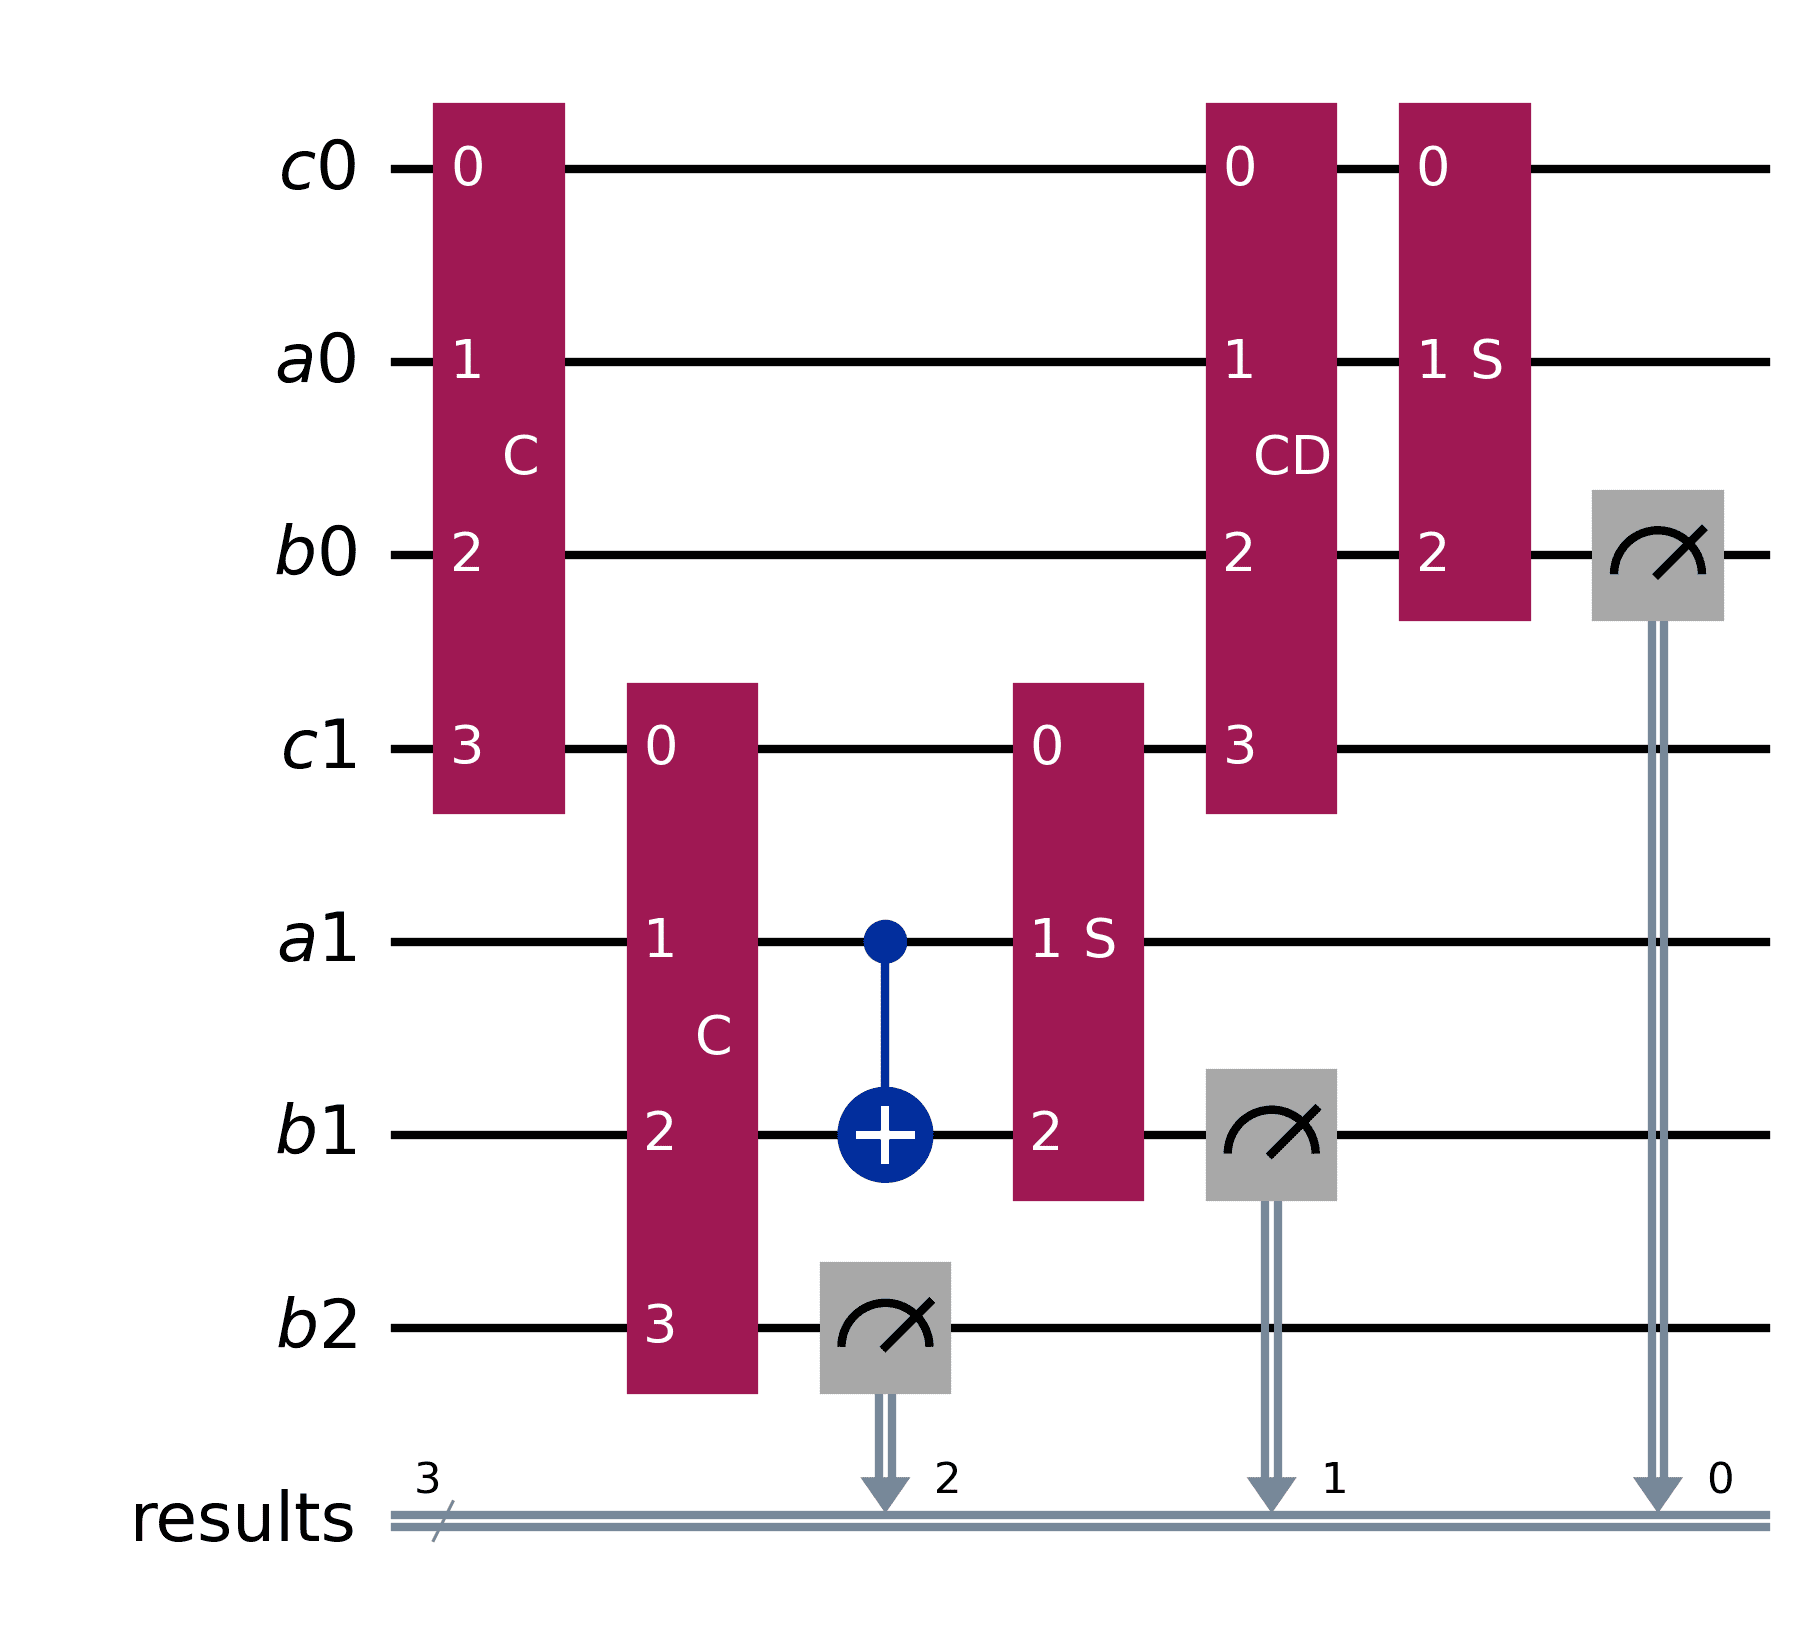
\includegraphics[width=0.6\textwidth]{adder}
    \caption{The adder circuit.}
    \label{fig:adder}
\end{figure}

The same adder circuit can be modified to include Shor code error correction at the very end. Gates are separately applied to every single physical qubit that makes up the logical qubit.  This results in the circuit shown in Figure \ref{fig:adder-corrected-end}.

\begin{figure}[H]
    \centering
    \includegraphics[width=\textwidth, height=9cm]{adder_corrected_end}
    \caption{The adder circuit with Shor code error correction at the end.}
    \label{fig:adder-corrected-end}
\end{figure}

Alternatively, the adder circuit can be modified to include Shor code error correction after every operation. This results in the circuit shown in Figure \ref{fig:adder-corrected-all-gates}.

\begin{figure}[H]
    \centering
    \includegraphics[width=\textwidth]{adder_corrected_all_gates}
    \caption{The adder circuit with Shor code error correction after every operation.}
    \label{fig:adder-corrected-all-gates}
\end{figure}

As with the previous circuits, the adder circuit can be extended for more bits by repeating the general structure. For all the circuits above, X gates were applied to qubits to set their initial state to 1 when necessary. Finally, the adder circuit can be modified to include transversal gates. This results in the circuit shown in Figure \ref{fig:adder-transversal}. Note that the X gates are replaced by Z gates and CNOT gates are replaced by flipped CNOT gates, as explained above.

\begin{figure}[H]
    \centering
    \includegraphics[width=\textwidth]{adder_transversal}
    \caption{The adder circuit with Shor code error correction after every operation and transversal gates. (Image rotated for better visibility.)}
    \label{fig:adder-transversal}
\end{figure}

\subsection{Running the Circuit}

Instead of running the circuit directly in the Jupyter notebooks, a Python class was created that would connect to IBM Quantum, run the circuit, and plot the results. This was done to reduce the amount of code duplication and to speed up development. The class could also be called with different parameters to run the circuit in different ways. The results were plotted using Matplotlib. The code for the class is situated in the file \texttt{notebooks/helpers/common.py} on Github.

\begin{lstlisting}[language=Python]
class RealQuantumComputer(QuantumComputer):
    def __init__(self, circuit: QuantumCircuit, shots: int = 128):
        super().__init__(circuit, shots)
        self.token = os.environ["IBM"]

        self.service = QiskitRuntimeService(channel="ibm_quantum", token=self.token)
        self.backend = self.service.least_busy(operational=True, simulator=False)

    def run(self, classical_name: str= "meas") -> dict:
        pm = generate_preset_pass_manager(backend=self.backend, optimization_level=1)
        isa_circuit = pm.run(self.circuit)

        sampler = SamplerV2(self.backend)
        job = sampler.run([isa_circuit], shots=self.shots)
        pub_result = job.result()[0]

        self.counts = pub_result.data[classical_name].get_counts()

        return self.counts

    def backend_name(self) -> str:
        return self.backend.name
\end{lstlisting}

For all the results below, the circuit was run on the IBM quantum computer ``ibm\_brisbane''. The circuit was run 512 times. Two four-bit qubits were added, 0010 and 0001. As such, the correct answer would be 00011.

\section{Results and Discussion}

\begin{figure}[H]
    \centering
    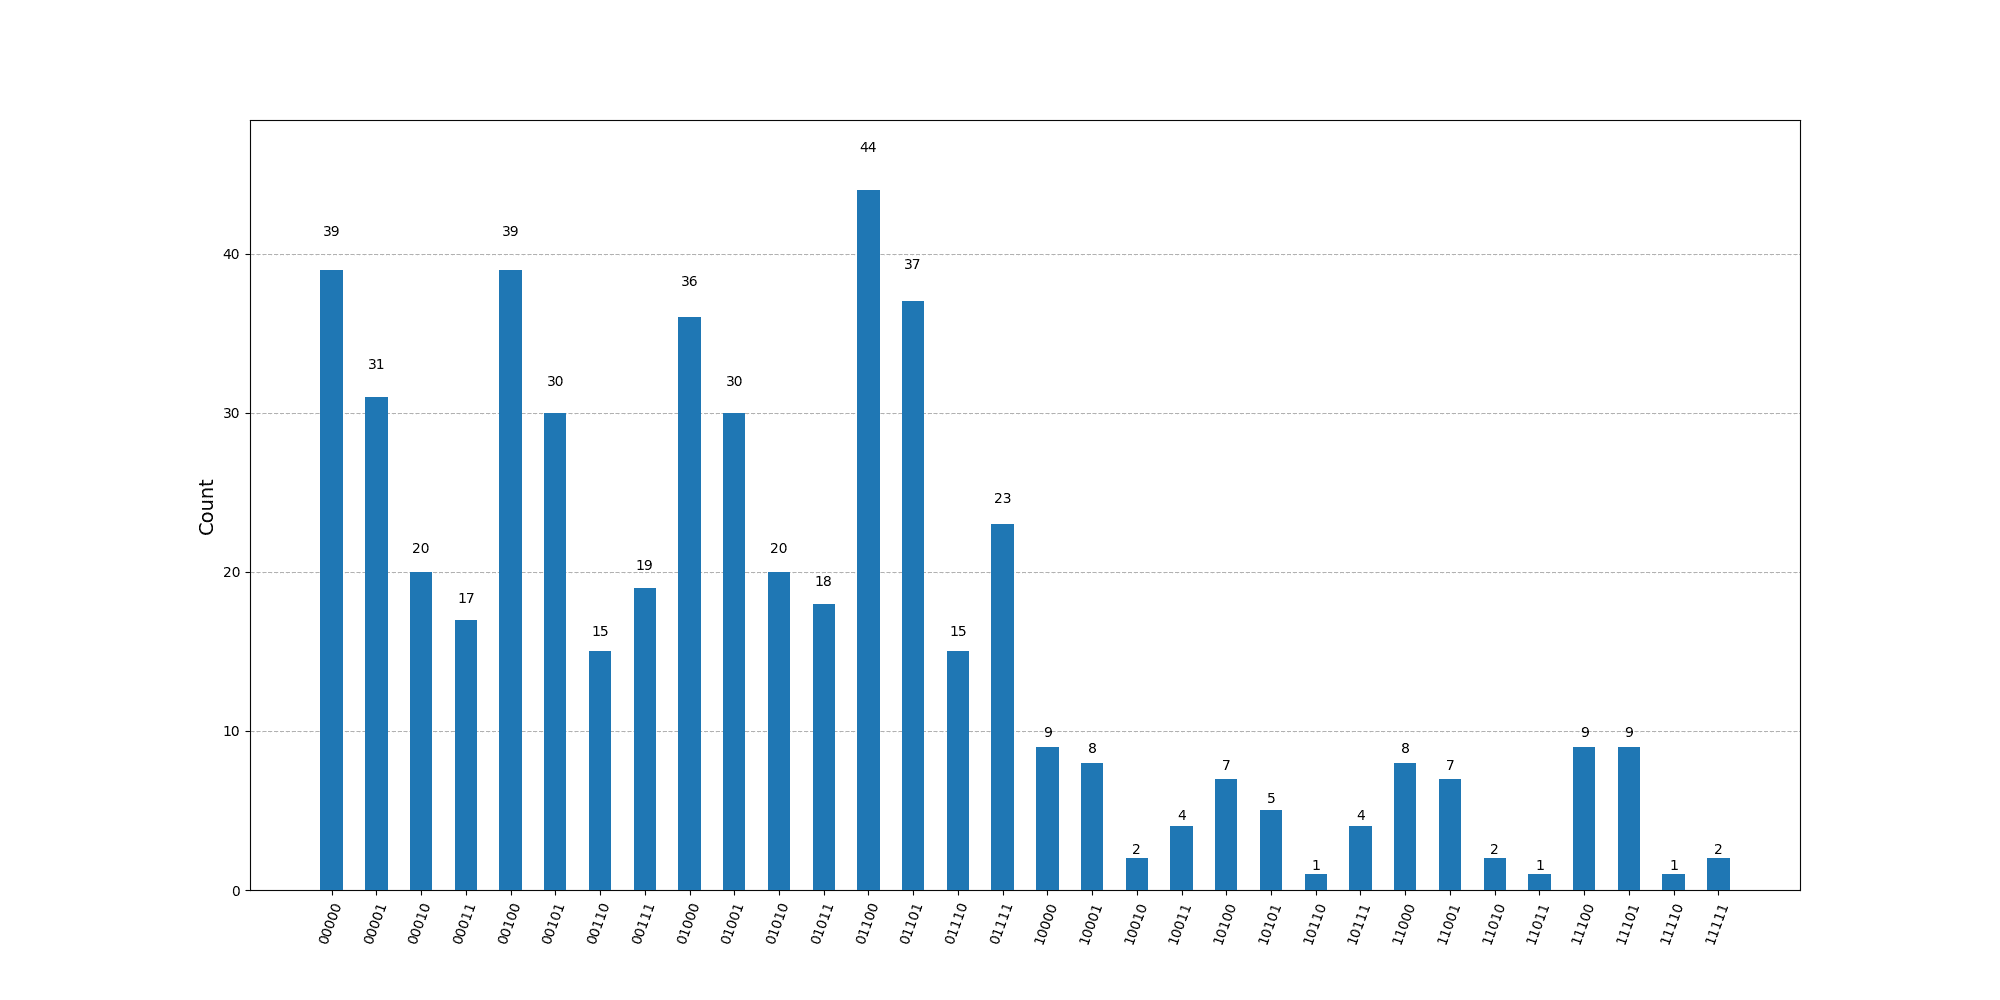
\includegraphics[width=\textwidth]{adder_plot}
    \caption{Plot of results with no error correction.}
    \label{fig:adder-plot}
\end{figure}

Running the adder circuit with no error correction lead to the results shown in Figure \ref{fig:adder-plot}. It did not give the correct answer, with the results mostly spread around the lower half of the possible answers. The correct answer had a 3.32\% chance of being produced.

\begin{figure}[H]
    \centering
    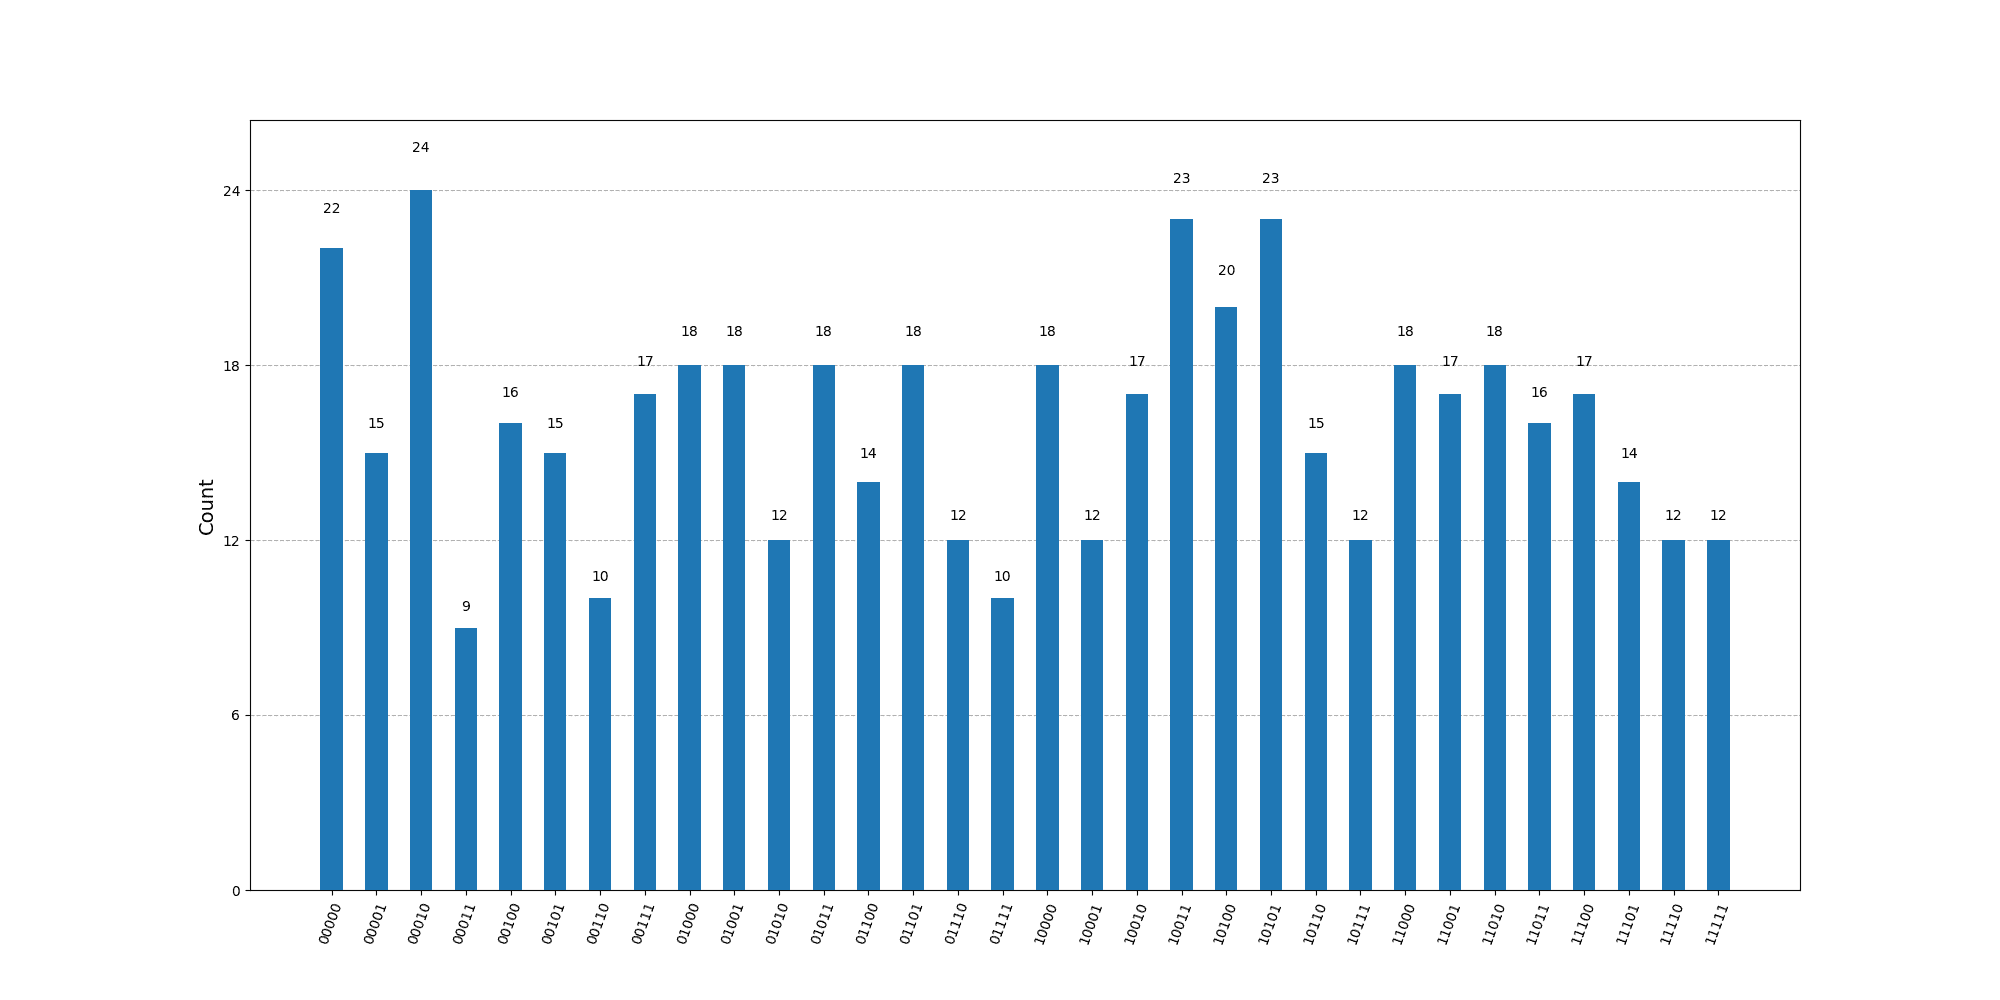
\includegraphics[width=\textwidth]{adder_corrected_end_plot}
    \caption{Plot of results applying the Shor code error correction at the end.}
    \label{fig:adder-corrected-end-plot}
\end{figure}

Running the circuit with Shor code error correction only at the end led to the results shown in Figure \ref{fig:adder-corrected-end-plot}. The results are worse than before, with an almost uniform distribution of results. The extra complexity from using nine times as many qubits meant that any errors were amplified, and as Shor code can only correct one qubit worth of errors, the results were worse. The correct answer had a 1.76\% chance of being produced.

\begin{figure}[H]
    \centering
    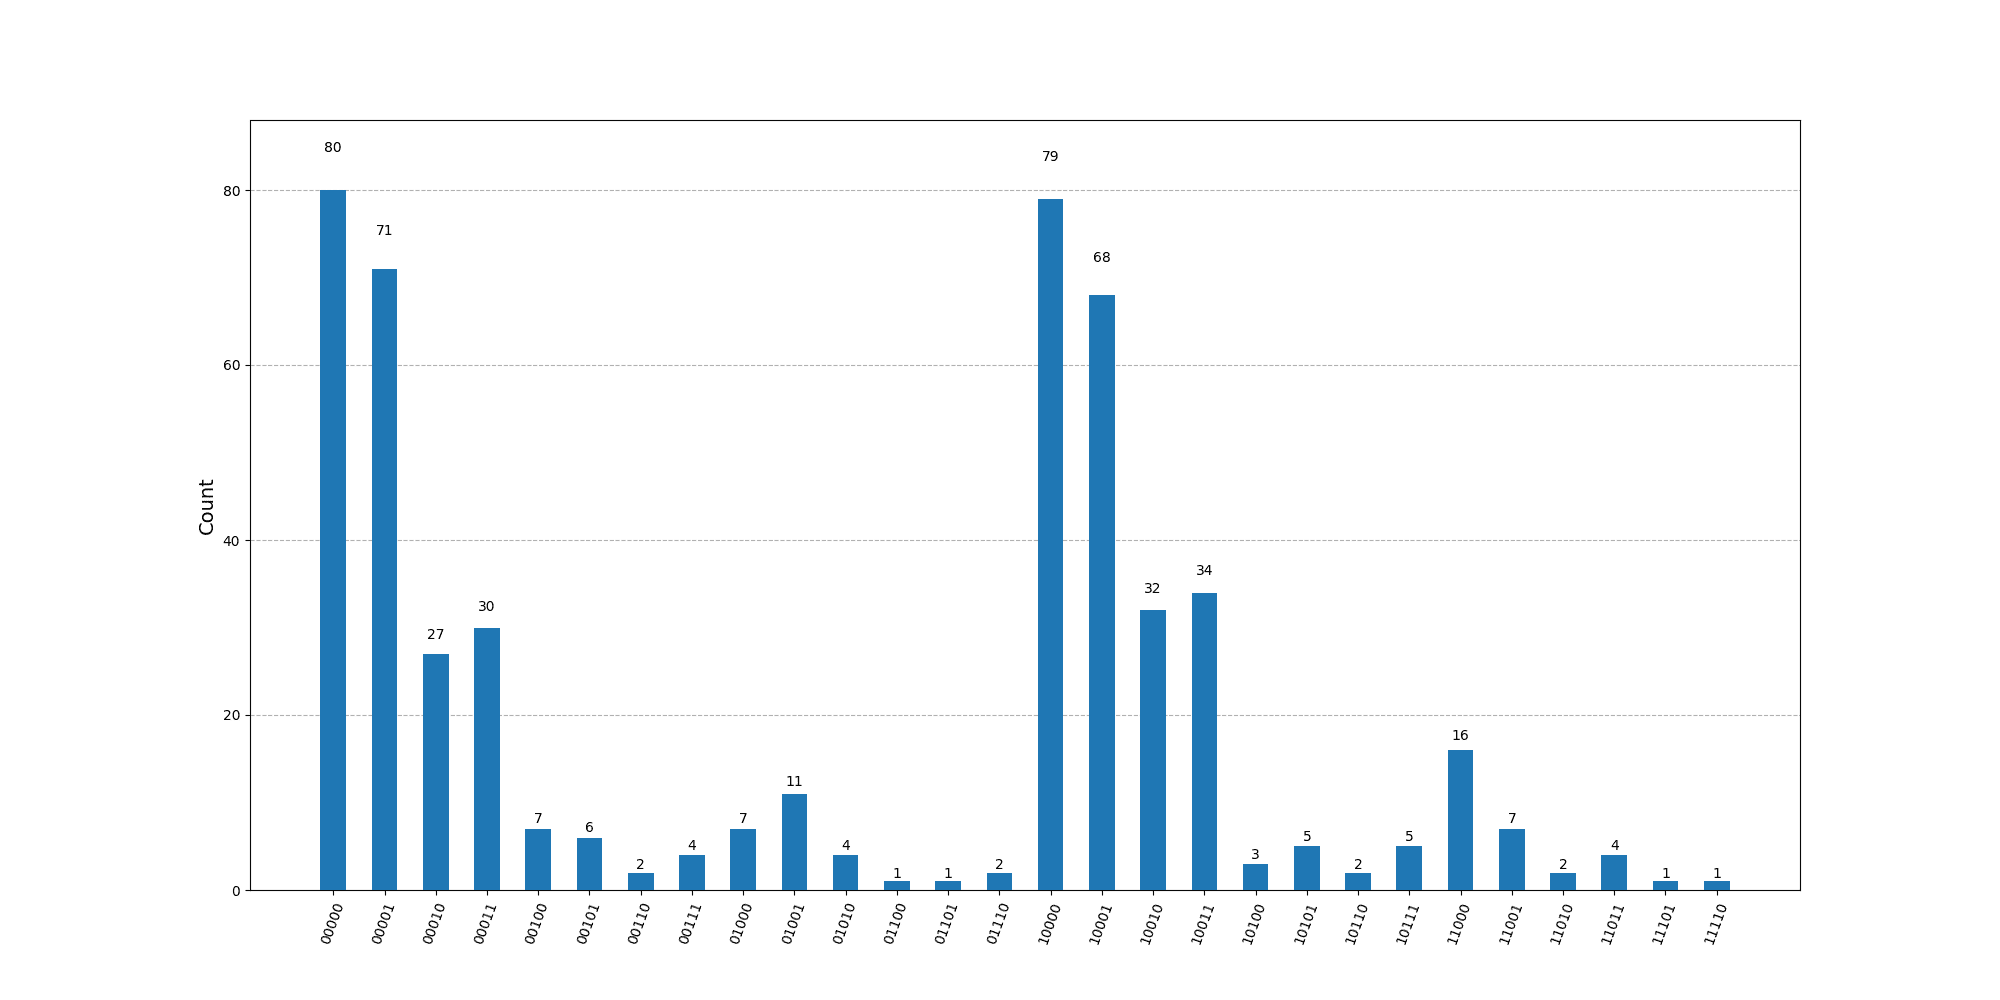
\includegraphics[width=\textwidth]{adder_corrected_all_gates_plot}
    \caption{Plot of results applying the Shor code error correction after every operation.}
    \label{fig:adder-corrected-all-gates-plot}
\end{figure}

Running the circuit with Shor code error correction after every operation led to the results shown in Figure \ref{fig:adder-corrected-all-gates-plot}. The results are better than before, with a more concentrated distribution of results. The results are centered around 00000 and 10000, which are still incorrect. There are smaller peaks at 00001 and 11000. The reason that the answers are concentrated at these two values is because the X gates used to set the initial values of the qubits are not transversal, and so did not actually change the values of the qubits. So the circuit was really adding 0000 and 0000, not 0010 and 0001. The correct answer had a 5.86\% chance of being produced.

\begin{figure}[H]
    \centering
    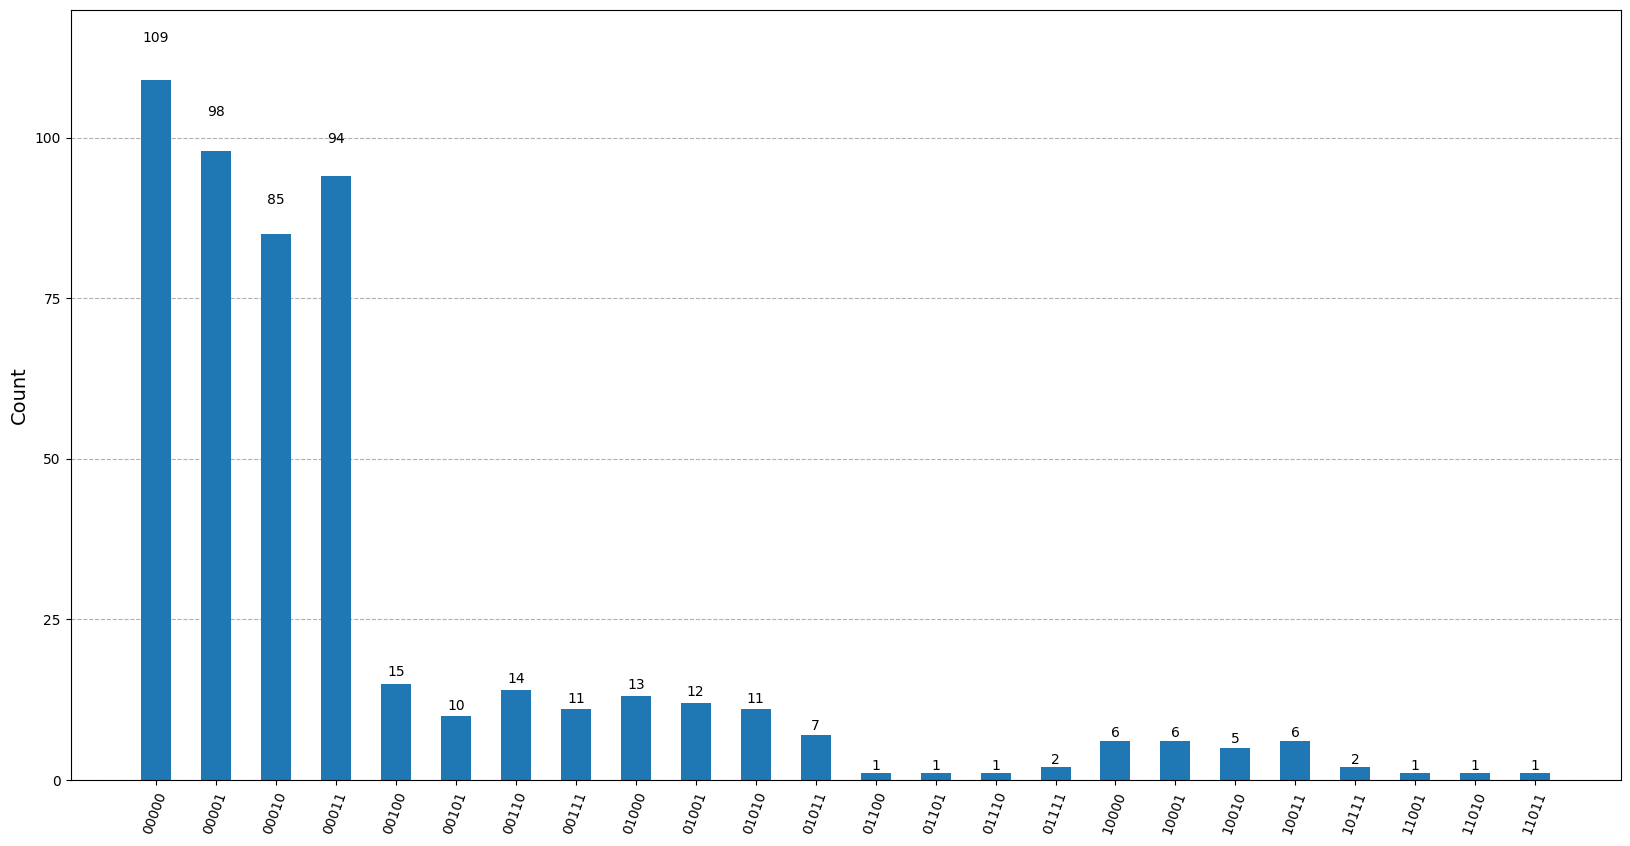
\includegraphics[width=0.8\textwidth]{adder_transversal_plot}
    \caption{Plot of results using transversal gates and Shor code error correction after every operation.}
    \label{fig:adder-transversal-plot}
\end{figure}

In order to actually add the correct numbers, the gates in the adder circuit must be replaced by their transversal versions. The X gates are replaced by Z gates, the CNOT by the flipped CNOT gates, etc. The results of running the circuit with transversal gates and Shor code error correction after every operation are shown in Figure \ref{fig:adder-transversal-plot}. The results are much better than the non-transversal version, but it still did not give the correct answer. The results are more concentrated around four values: 00000, 00001, 00010, and 00011, with no other peaks. The correct answer had a 16.6\% chance of being produced, which is the highest of all the results, by a significant margin.

\section{Conclusion}

The results show that the Shor code error correction was effective in correcting errors in the adder circuit. However, the results were not perfect. The main reason for this is that the CNOT and Toffoli gates used in the adder circuit need to be converted to their transversal version. While the non-transversal version had a higher chance to give the correct answer, this could also just be a result of run-to-run variation.

The Shor code was effective in correcting errors in the adder circuit. However, the gates in the adder circuit need to be converted to their transversal versions in order to get the correct results. The Shor code was most effective when applied after every operation in the circuit. Using the Shor code only at the end of the entire circuit was the only time worse results were produced. The extra complexity from using nine times as many qubits was greater than the error correction provided by the Shor code. The results show that the Shor code is not perfect. The chance of getting the incorrect answer is high enough that this circuit should not be used in a real-world application.

Future work could involve implementing the Toffoli gate in a transversal way. This would allow the adder circuit to be run with the Shor code error correction after every operation, which was the most effective way of using the Shor code. The results could be improved by using a more advanced error correction code, such as the surface code, which can correct multiple qubit errors. Work should also be done to reduce the variation that occurs between runs of the circuit.

\end{document}
